\chapter{State Machines}\label{state_machine_chap}

State machines are a simple, abstract model of step-by-step processes.
Since computer programs can be understood as defining step-by-step
computational processes, it's not surprising that state machines come
up regularly in computer science.  They also come up in many other
settings such as designing digital circuits and modeling probabilistic
processes.  This section introduces \emph{Floyd's Invariant Principle}
which is a version of induction tailored specifically for proving
properties of state machines.

\iffalse
You may already have seen them in a digital logic course,
a compiler course, or a probability course.
\fi

One of the most important uses of induction in computer science
involves proving one or more desirable properties continues to hold at
every step in a process.  A property that is preserved through a
series of operations or steps is known as a \emph{preserved
  invariant}.\index{invariant}\index{preserved
  invariant|see{invariant}}

Examples of desirable invariants include properties such as the
altitude of a plane remaining above 1,000 feet unless the wingflaps
\iffalse and landing gear\fi are deployed, or the temperature of a
nuclear reactor remaining below the meltdown threshold.

\iffalse  %%FTL
In particular, we show that the proposition is true at the beginning
(this is the base case) and that if it is true after $t$ steps have
been taken, it will also be true after step~$t + 1$ (this is the
inductive step).  We can then use the induction principle to conclude
that the proposition is indeed an invariant, namely, that it will
always hold.
\fi

\section{States and Transitions}

Formally, a \term{state machine} is nothing more than a \idx{binary
  relation} on a set, except that the elements of the set are called
``states,'' the relation is called the transition relation, and an
arrow in the graph of the transition relation is called a
\emph{transition}.  A transition from state $q$ to state $r$ will be
written $q \movesto r$.  The transition relation is also called the
\emph{state graph} of the machine.  A state machine also comes
equipped with a designated \emph{start state}.

A simple example is a bounded counter, which counts from $0$ to $99$
and overflows at 100.  This state machine is pictured in
Figure~\ref{fig:counter}, with states pictured as circles, transitions
by arrows, and with start state 0 indicated by the double circle.
\begin{figure}
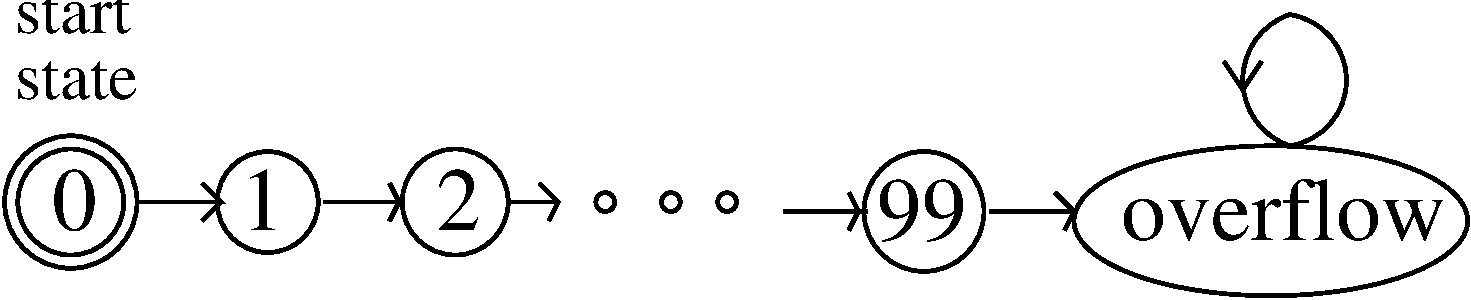
\includegraphics[width = 3in]{counter}
\caption{\em State transitions for the 99-bounded counter.}
\label{fig:counter}
\end{figure}
To be precise, what the picture tells us is that this bounded counter machine has
\begin{align*}
\text{states} &  \eqdef \set{0, 1,\dots,99, \text{overflow}},\\
\text{start state}  & \eqdef 0,\\
\text{transitions} & \eqdef \set{n \movesto n+1 \suchthat 0 \le n < 99}\\
                   &\quad  \union \set{99 \movesto \text{overflow},
                                 \text{overflow} \movesto \text{overflow}}.
\end{align*}
This machine isn't much use once it overflows, since it has no way to
get out of its overflow state.

State machines for digital circuits and string pattern matching
algorithms, for instance, usually have only a finite number of states.
Machines that model continuing computations typically have an infinite
number of states.  For example, instead of the 99-bounded counter, we
could easily define an ``unbounded'' counter that just keeps counting
up without overflowing.  The unbounded counter has an infinite state
set, the nonnegative integers, which makes its state diagram
harder to draw.

State machines are often defined with labels on states and/or transitions
to indicate such things as input or output values, costs, capacities, or
probabilities.  Our state machines don't include any such labels because
they aren't needed for our purposes.  We do name states, as in
Figure~\ref{fig:counter}, so we can talk about them, but the names aren't
part of the state machine.

\section{The Invariant Principle}

\subsection{A Diagonally-Moving Robot}
Suppose we have a robot that starts at the origin and moves on an
infinite 2-dimensional integer grid.  The \emph{state} of the robot at
any time can be specified by the integer coordinates $(x, y)$ of the
robot's current position.  So the \emph{start state} is~$(0, 0)$.  At
each step, the robot may move to a diagonally adjacent grid point, as
illustrated in Figure~\ref{fig:diagrobot}.

\begin{figure}
\graphic{Fig_robot-a}
\caption{\em The Diagonally Moving Robot.}
\label{fig:diagrobot}
\end{figure}

To be precise, the robot's transitions are:
\[
\set{(m,n)\movesto (m\pm 1, n\pm 1) \suchthat m,n \in \integers}.
\]
For example, after the first step, the robot could be in states $(1,
1)$, $(1, -1)$, $(-1, 1)$ or $(-1, -1)$.  After two steps, there are
9 possible states for the robot, including~$(0, 0)$.
The question is, can the robot ever reach position~$(1, 0)$?

\begin{figure}
\graphic{Fig_robot-b}
\caption{\em Can the Robot get to $(1,0)$?}
\label{fig:robot-to10}
\end{figure}

If you play around with the robot a bit, you'll probably notice that
the robot can only reach positions~$(m, n)$ for which $m + n$ is even,
which of course means that it can't reach $(1,0)$.  This follows
because the evenness of the sum of the coordinates is a property that
is \emph{preserved} by transitions.  This is an example of a
\term{preserved invariant}\index{invariant}.

This once, let's go through this preserved invariant argument,
carefully highlighting where induction comes in.  Specifically, define
the even-sum property of states to be:
\[
\text{Even-sum}((m,n)) \eqdef [m+n \text{ is even}].
\]
\begin{lemma}\label{even-sum-invar}
For any transition $q \movesto r$ of the diagonally-moving robot, if
Even-sum($q$), then Even-sum($r$).
\end{lemma}
This lemma follows immediately from the definition of the robot's
transitions: $(m,n)\movesto (m\pm 1, n\pm 1)$.  After a transition,
the sum of coordinates changes by $(\pm 1) + (\pm 1)$, that is, by 0,
2, or -2.  Of course, adding 0, 2 or -2 to an even number gives an
even number.  So by a trivial induction on the number of transitions,
we can prove:
\begin{theorem}\label{th:diag-robot}
The sum of the coordinates of any state reachable by the
diagonally-moving robot is even.
\end{theorem}

\begin{proof}
The proof is induction on the number of transitions the robot has
made.  The induction hypothesis is
\[
P(n) \eqdef \text{if $q$ is a state reachable in $n$ transitions, then
  Even-sum($q$)}.
\]

\inductioncase{Base case}: $P(0)$ is true since the only state reachable in 0
transitions is the start state $(0, 0)$, and $0 + 0$ is even.

\inductioncase{Inductive step}: Assume that $P(n)$ is true, and let $r$ be any
state reachable in $n+1$ transitions. We need to prove that
Even-sum($r$) holds.

Since $r$ is reachable in $n+1$ transitions, there must be a state
$q$ reachable in $n$ transitions such that $q \movesto r$.  Since
$P(n)$ is assumed to be true, Even-sum($q$) holds, and so by
Lemma~\ref{even-sum-invar}, Even-sum($r$) also holds.  This proves
that $P(n) \QIMPLIES P(n + 1)$ as required, completing the proof of
the inductive step.

We conclude by induction that for all $n \ge 0$, if $q$ is reachable
in $n$ transitions, then Even-sum($q$).  This implies that every
reachable state has the Even-sum property.

\end{proof}

\begin{corollary}\label{cor:diag-robot}
The robot can never reach position~$(1, 0)$.
\end{corollary}

\begin{proof}
By Theorem~\ref{th:diag-robot}, we know the robot can only reach
positions with coordinates that sum to an even number, and thus it
cannot reach position~$(1, 0)$.
\end{proof}

\iffalse
Since this was the first time we proved that a predicate was an
invariant, we were careful to go through all four cases in gory
detail.  As you become more experienced with such proofs, you will
likely become more brief as well.  Indeed, if we were going through
the proof again at a later point in the text, we might simply note
that the sum of the coordinates after step~$t + 1$ can be only $x +
y$, $x + y + 2$ or $x + y - 2$ and therefore that the sum is even.
%%FTL
\fi

\subsection{Statement of the Invariant Principle}\label{subsec:invariant}
Using the Even-sum invariant to understand the diagonally-moving robot
is a simple example of a basic proof method called The Invariant
Principle.  The Principle summarizes how induction on the number of
steps to reach a state applies to invariants.   

\iffalse

To formulate it precisely, we need a definition of
\term{reachability.}

\begin{definition}
The \term{reachable states} of a state machine $M$ are defined
recursively as follows:
\begin{itemize}
\item the start state is reachable, and
\item if $p$ is a reachable state of $M$, and $p \movesto q$ is a
  transition of $M$, then $q$ is also a reachable state of $M$.
\end{itemize}
\end{definition}
\fi

A state machine \emph{execution} describes a possible sequence of
steps a machine might take.

\begin{definition}
An \emph{execution}%
\index{state machine!execution} 
of the state machine is a (possibly infinite)
sequence of states with the property that
\begin{itemize}
\item it begins with the start state, and
\item if $q$ and $r$ are consecutive states in the sequence, then $q
  \movesto r$.
\end{itemize}
A state is called \term{reachable} if it appears in some execution.
\end{definition}

\begin{definition}
  A \emph{preserved} \term{invariant}
%\index{invariant|seealso{state machine}} 
of a state machine is a predicate $P$ on
  states, such that whenever $P(q)$ is true of a state $q$ and $q
  \movesto r$ for some state $r$ then $P(r)$ holds.
\end{definition}

\textbox{
\textboxheader{The Invariant Principle}

\noindent If a preserved invariant of a state machine is true for the
start state,\\
then it is true for all reachable states.}

\index{invariant!Invariant Principle}

The Invariant Principle is nothing more than the Induction Principle
reformulated in a convenient form for state machines.  Showing that a
predicate is true in the start state is the base case of the
induction, and showing that a predicate is a preserved invariant
corresponds to the inductive step.\footnote{Preserved invariants are
  commonly just called ``invariants'' in the literature on program
  correctness, but we decided to throw in the extra adjective to avoid
  confusion with other definitions.  For example, other texts (as well
  as another subject at MIT) use ``invariant'' to mean ``predicate
  true of all reachable states.''  Let's call this definition
  ``invariant-2.''  Now invariant-2 seems like a reasonable
  definition, since unreachable states by definition don't matter, and
  all we want to show is that a desired property is invariant-2.  But
  this confuses the \emph{objective} of demonstrating that a property
  is invariant-2 with the \emph{method} of finding a \emph{preserved}
  invariant---which is preserved even at unreachable states---to
  \emph{show} that it is invariant-2.}

\textbox{
\textboxheader{Robert W. Floyd}
\begin{center}
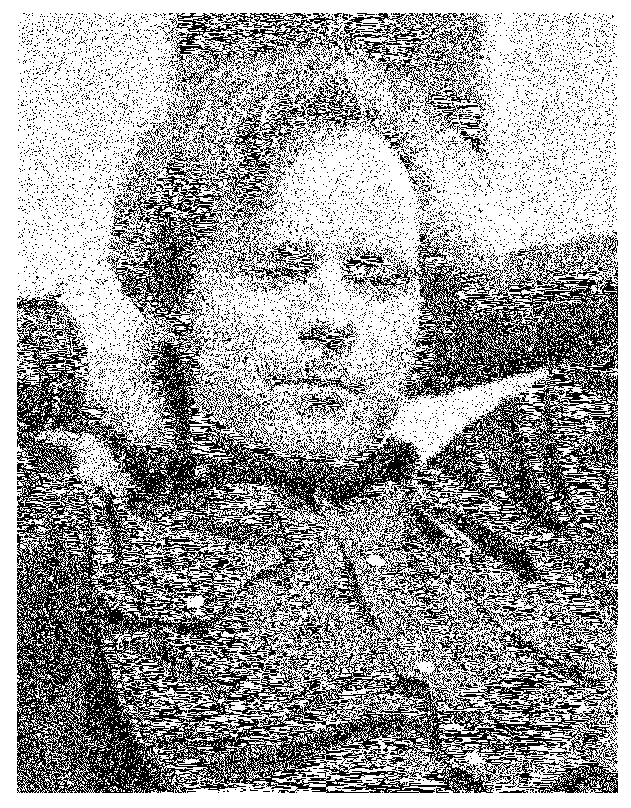
\includegraphics[width = 2in]{floyd72}
\end{center}

The Invariant Principle was formulated by Robert W. Floyd%
\index{Floyd, Robert W.}  at Carnegie Tech in 1967. (Carnegie Tech was
renamed Carnegie-Mellon University the following year.)  Floyd was
already famous for work on the formal grammars that transformed the
field of programming language parsing; that was how he got to be a
professor even though he never got a Ph.D.  (He had been admitted to a
PhD program as a teenage prodigy, but flunked out and never went
back.)

In that same year, Albert R. Meyer%
\index{Meyer, Albert R} 
was appointed Assistant Professor in the Carnegie Tech Computer
 Science Department, where he
first met Floyd.  Floyd and Meyer were the only theoreticians in the
department, and they were both delighted to talk about their shared
interests.  After just a few conversations, Floyd's new junior
colleague decided that Floyd was the smartest person he had ever met.

Naturally, one of the first things Floyd wanted to tell Meyer about was
his new, as yet unpublished, Invariant Principle.  Floyd explained the
result to Meyer, and Meyer wondered (privately) how someone as brilliant
as Floyd could be excited by such a trivial observation.  Floyd had to
show Meyer a bunch of examples before Meyer understood Floyd's excitement
---not at the truth of the utterly obvious Invariant Principle, but rather
at the insight that such a simple method could be so widely and easily
applied in verifying programs.

Floyd left for Stanford the following year.  He won the Turing
award---the ``Nobel prize'' of computer science---in the late 1970's,
in recognition of his work on grammars and on the foundations of
program verification.  He remained at Stanford from 1968 until his
death in September, 2001.  You can learn more about Floyd's life and
work by reading the
\href{http://courses.csail.mit.edu/6.042/spring13/floyd-eulogy-by-knuth.pdf}{eulogy}
at
\begin{center}
   \href{http://oldwww.acm.org/pubs/membernet/stories/floyd.pdf}
        {http://oldwww.acm.org/pubs/membernet/stories/floyd.pdf}
\end{center}
written by his closest colleague, Don Knuth.
}

\subsection{The Die Hard Example}\label{diehard_example}
The movie \textit{Die Hard 3: With a Vengeance} includes an amusing
example of a state machine.  The lead characters played by Samuel
L. Jackson and Bruce Willis have to disarm a bomb planted by the
diabolical Simon Gruber:

\textbox{
\begin{list}{}{\itemsep=0in \leftmargin=0.25in \rightmargin=0.25in}

\item[\textbf{Simon:}] On the fountain, there should be 2 jugs, do you
see them?  A 5-gallon and a 3-gallon.  Fill one of the jugs with
exactly 4 gallons of water and place it on the scale and the timer
will stop.  You must be precise; one ounce more or less will result in
detonation.  If you're still alive in 5 minutes, we'll speak.

\item[\textbf{Bruce:}] Wait, wait a second. I don't get it. Do you get it?

\item[\textbf{Samuel:}] No.

\item[\textbf{Bruce:}] Get the jugs.  Obviously, we can't fill the 3-gallon jug
with 4 gallons of water.

\item[\textbf{Samuel:}] Obviously.

\item[\textbf{Bruce:}] All right.  I know, here we go.  We fill the
  3-gallon jug exactly to the top, right?

\item[\textbf{Samuel:}] Uh-huh.

\item[\textbf{Bruce:}] Okay, now we pour this 3 gallons into the 5-gallon jug,
giving us exactly 3 gallons in the 5-gallon jug, right?

\item[\textbf{Samuel:}] Right, then what?

\item[\textbf{Bruce:}] All right. We take the 3-gallon jug and fill it a third
of the way...

\item[\textbf{Samuel:}] No!  He said, ``Be precise.''  Exactly 4
gallons.

\item[\textbf{Bruce:}] Sh - -.  Every cop within 50 miles is running his a - - off
and I'm out here playing kids games in the park.

\item[\textbf{Samuel:}] Hey, you want to focus on the problem at hand?

\end{list}
}

Fortunately, they find a solution in the nick of time.  You can work out
how.

\subsubsection{The Die Hard 3 State Machine}\label{diehard_machine}
The jug-filling scenario can be modeled with a state machine that keeps
track of the amount $b$ of water in the big jug, and the amount $l$
in the little jug.  With the 3 and 5 gallon water jugs, the states
formally will be pairs $(b,l)$ of real numbers such that $0 \leq b \leq
5, 0 \leq l \leq 3$.  (We can prove that the reachable values of $b$ and
$l$ will be nonnegative integers, but we won't assume this.)  The start
state is $(0,0)$, since both jugs start empty.

Since the amount of water in the jug must be known exactly, we will only
consider moves in which a jug gets completely filled or completely
emptied.  There are several kinds of transitions:
\begin{enumerate}

\item  Fill the little jug: $(b,l) \movesto (b,3)$ for $l < 3$.

\item  Fill the big jug: $(b,l) \movesto (5,l)$ for $b<5$.

\item  Empty the little jug: $(b,l) \movesto (b,0)$ for $l>0$.

\item  Empty the big jug: $(b,l) \movesto (0,l)$ for $b>0$.

\item  Pour from the little jug into the big jug: for $l>0$,
\begin{equation*}
(b,l) \movesto
\begin{cases}
(b+l, 0) & \text{if $b + l \le 5$,}\\
(5, l - (5 - b)) & \text{otherwise.}
\end{cases}
\end{equation*}

\item Pour from big jug into little jug: for $b>0$,
\begin{equation*}
(b,l) \movesto
\begin{cases}
(0, b+l) & \text{if $b + l \le 3$,}\\
(b - (3 -l), 3) & \text{otherwise.}
\end{cases}
\end{equation*}
\end{enumerate}

Note that in contrast to the 99-counter state machine, there is more than
one possible transition out of states in the Die Hard machine.  Machines
like the 99-counter with at most one transition out of each state are
called \emph{deterministic}.  The Die Hard machine is
\emph{nondeterministic} because some states have transitions to several
different states.

The Die Hard 3 bomb gets disarmed successfully because the state (4,3)
is reachable.

%\end{example}

%\subsubsection{Reachability and Preserved Invariants}

\subsubsection{Die Hard Permanently}
The \emph{Die Hard} series is getting tired, so we propose a final
\emph{Die Hard Permanently}.  Here, Simon's brother returns to
avenge him, posing the same challenge, but with the 5 gallon jug
replaced by a 9 gallon one.  The state machine has the same
specification as the Die Hard 3 version, except all occurrences of
``5'' are replaced by ``9.''

Now, reaching any state of the form $(4,l)$ is impossible.  We prove
this using the Invariant Principle.  Specifically, we define the
preserved invariant predicate $P((b,l))$ to be that $b$ and $l$ are
nonnegative integer multiples of 3.

To prove that $P$ is a preserved invariant of Die-Hard-Once-and-For-All
machine, we assume $P(q)$ holds for some state $q \eqdef (b,l)$ and that
$q \movesto r$.  We have to show that $P(r)$ holds.  The proof divides
into cases, according to which transition rule is used.

One case is a ``fill the little jug'' transition.  This means $r =
(b,3)$.  But $P(q)$ implies that $b$ is an integer multiple of 3, and
of course 3 is an integer multiple of 3, so $P(r)$ still holds.

Another case is a ``pour from big jug into little jug'' transition.
For the subcase when there isn't enough room in the little jug to hold
all the water, that is, when $b + l > 3$, we have $r = (b -( 3 -l), 3)$.
But $P(q)$ implies that $b$ and $l$ are integer multiples of 3, which
means $b -( 3 -l)$ is too, so in this case too, $P(r)$ holds.

We won't bother to crank out the remaining cases, which can all be checked
just as easily.  Now by the Invariant Principle, we conclude that every
reachable state satisifies $P$.  But since no state of the form $(4,l)$
satisifies $P$, we have proved rigorously that Bruce dies once and for
all!

By the way, notice that the state (1,0), which satisfies $\QNOT(P)$, has a
transition to (0,0), which satisfies $P$.  So the negation of a preserved
invariant may not be a preserved invariant.

\section{Partial Correctness \& Termination}\label{partial_correct_sec}

Floyd distinguished two required properties to verify a program.  The
first property is called \term{partial correctness}; this is the property
that the final results, if any, of the process must satisfy system
requirements.

You might suppose that if a result was only partially correct, then it
might also be partially incorrect, but that's not what Floyd meant.  The
word ``partial'' comes from viewing a process that might not terminate as
computing a \emph{partial relation}.  Partial correctness means that
\emph{when there is a result}, it is correct, but the process might not
always produce a result, perhaps because it gets stuck in a loop.

The second correctness property, called%
\index{termination (state machine)|textbf}
\emph{termination}, is that the
process does always produce some final value.

Partial correctness can commonly be proved using the Invariant Principle.
Termination can commonly be proved using the \idx{Well Ordering Principle}.
We'll illustrate this by verifying a Fast Exponentiation procedure.

\subsection{Fast Exponentiation}\label{fast_exp_subsec}

\subsubsection{Exponentiating}\label{fast_exp_subsubsec}
The most straightforward way to compute the $b$th power of a number
$a$ is to multiply $a$ by itself $b-1$ times.  But the solution can
be found in considerably fewer multiplications by using a technique
called \term{Fast Exponentiation}.  The register machine program below
defines the fast exponentiation algorithm.  The letters $x,y,z,r$
denote registers that hold numbers. An \emph{assignment statement} has
the form ``$z := a$'' and has the effect of setting the number in
register $z$ to be the number $a$.

\textbox{
\textboxheader{A Fast Exponentiation Program}

Given inputs $a \in \reals, b \in \nngint$,
initialize registers $x,y,z$ to $a,1,b$ respectively,
and repeat the following sequence of steps until termination:
\begin{itemize}\renewcommand{\itemsep}{0pt}
\item if $z = 0$ \textbf{return} $y$ and terminate
\item $r := \text{remainder}(z,2)$
\item $z := \quotient(z,2)$
\item if $r = 1$, then $y := xy$
\item $x := x^2$
\end{itemize}
}

We claim this program always terminates and leaves $y = a^b$.

To begin, we'll model the behavior of the program with a state
machine:
\begin{enumerate}
\item $\text{states} \eqdef \reals \cross \reals \cross \nngint$,
\item $\text{start state} \eqdef (a,1,b)$,
\item transitions are defined by the rule
\begin{equation*}
(x,y,z) \movesto
\begin{cases}
(x^2, y, \quotient(z,2)) & \text{if $z$ is nonzero and even},\\
(x^2, xy, \quotient(z,2)) & \text{if $z$ is nonzero and odd}.
\end{cases}
\end{equation*}
\end{enumerate}

The preserved invariant $P((x,y,z))$ will be
\begin{equation}\label{yxzd}
z \in \nngint \QAND yx^z = a^b.
\end{equation}

To prove that $P$ is preserved, assume $P((x,y,z))$ holds
and that $(x,y,z) \movesto (x_t,y_t,z_t)$.  We must prove that
$P((x_t,y_t,z_t))$ holds, that is,
\begin{equation}\label{ztytxt}
z_t \in \nngint \QAND y_tx_t^{z_t} = a^b.
\end{equation}

Since there is a transition from $(x,y,z)$, we have $z \neq 0$, and since
$z \in \nngint$ by~\eqref{yxzd}, we can consider just two cases:

If $z$ is even, then we have that $x_t = x^2, y_t = y, z_t = z/2$.
Therefore, $z_t \in \nngint$ and
\begin{align*}
y_tx_t^{z_t} & = y(x^2)^{z/2}\\
           & = yx^{2\cdot z/2}\\
           & = yx^z\\
           & = a^b & \mbox{(by~\eqref{yxzd})}
\end{align*}

If $z$ is odd, then we have that $x_t = x^2, y_t = xy, z_t = (z-1)/2$.
Therefore, $z_t \in \nngint$ and
\begin{align*}
y_tx_t^{z_t} & = xy(x^2)^{(z-1)/2}\\
& = yx^{1+2 \cdot (z-1)/2}\\
& = yx^{1+(z-1)}\\
& = yx^z\\
& = a^b & \mbox{(by~\eqref{yxzd})}
\end{align*}

So in both cases,~\eqref{ztytxt} holds, proving that $P$ is a preserved
invariant.

Now it's easy to prove partial correctness: if the Fast
Exponentiation program terminates, it does so with $a^b$ in register
$y$.  This works because $1\cdot a^b = a^b$, which means
that the start state $(a,1,b)$ satisifies $P$.  By the Invariant
Principle, $P$ holds for all reachable states.  But the program
only stops when $z = 0$.  If a terminated state $(x,y,0)$ is
reachable, then $y = yx^0 = a^b$ as required.

Ok, it's partially correct, but what's fast about it?  The answer is
that the number of multiplications it performs to compute $a^b$ is
roughly the length of the binary representation of $b$.  That is, the
Fast Exponentiation program uses roughly $\log b$\footnote{As usual in
  computer science, $\log b$ means the base two logarithm $\log_2 b$.
  We use, $\ln b$ for the natural logarithm $\log_e b$, and otherwise
  write the logarithm base explicitly, as in $\log_{10} b$.}
 multiplications,
compared to the naive approach of multiplying by $a$ a total of $b-1$
times.

More precisely, it requires at most $2 (\ceil{\log b}+1)$
multiplications for the Fast Exponentiation algorithm to compute $a^b$ for
$b>1$.  The reason is that the number in register $z$ is initially $b$,
and gets at least halved with each transition.  So it can't be halved more
than $\ceil{\log b}+1$ times before hitting zero and causing the
program to terminate.  \iffalse The $(b+1)$ comes in because for $b =
2^p$, a power of two, it takes $(p+1)$ halves to get zero.  \fi Since each
of the transitions involves at most two multiplications, the total number
of multiplications until $z=0$ is at most $2(\ceil{\log b}+1)$ for $b
> 0$ (see Problem~\ref{PS_2logb_mults}).

\subsection{Derived Variables}\label{derived_var_subsec}

The preceding termination proof involved finding a nonnegative
integer-valued measure to assign to states.  We might call this measure
the ``size'' of the state.  We then showed that the size of a state
decreased with every state transition.  By the Well Ordering Principle,
the size can't decrease indefinitely, so when a minimum size state is
reached, there can't be any transitions possible: the process has
terminated.

More generally, the technique of assigning values to states---not
necessarily nonnegative integers and not necessarily decreasing under
transitions---is often useful in the analysis of algorithms.
\emph{Potential functions} play a similar role in physics.  In the
context of computational processes, such value assignments for states
are called \term{derived variables}.

For example, for the Die Hard machines we could have introduced a derived
variable $f:\text{states} \to \reals$ for the amount of water in both
buckets, by setting $f((a, b)) \eqdef a + b$.  Similarly, in the robot
problem, the position of the robot along the $x$-axis would be given by
the derived variable $x\text{-coord}$, where $x\text{-coord}((i, j))
\eqdef~i$.

%\subsubsection{Weakly Decreasing Variables}

There are a few standard properties of derived variables that are handy in
analyzing state machines.

\begin{definition}
  A derived variable $f:\text{states} \to \reals$ is \term{strictly
    decreasing} iff
\[
q \movesto q' \QIMP\ f(q') < f(q).
\]
It is \term{weakly decreasing} iff
\[
q \movesto q' \QIMP\ f(q') \leq f(q).
\]

\emph{Strictly increasing}% \index{strictly increasing|textbf} and
\term{weakly increasing} derived variables are defined
similarly.\footnote{Weakly increasing variables are often also called
  \emph{nondecreasing}.  We will avoid this terminology to prevent
  confusion between nondecreasing variables and variables with the
  much weaker property of \emph{not} being a decreasing variable.}
\end{definition}

We confirmed termination of the Fast Exponentiation procedure by
noticing that the derived variable $z$ was nonnegative-integer-valued
and strictly decreasing.  We can summarize this approach to proving
termination as follows:
\begin{theorem}\label{th:decr}
If $f$ is a strictly decreasing $\nngint$-valued derived variable of a
state machine, then the length of any execution starting at state $q$ is
at most $f(q)$.
\end{theorem}

Of course, we could prove Theorem~\ref{th:decr} by induction on the value
of $f(q)$, but think about what it says: ``If you start counting down at
some nonnegative integer $f(q)$, then you can't count down more than
$f(q)$ times.''  Put this way, it's obvious.


\subsection{Termination with Well ordered Sets (Optional)}

Theorem~\ref{th:decr} generalizes straightforwardly to derived
variables taking values in a well ordered set
(Section~\ref{well_ordering_sec}.

\begin{theorem}\label{well_order_decreasing}
  If there exists a strictly decreasing derived variable whose range
  is a well ordered set, then every execution terminates.
\end{theorem}

Theorem~\ref{well_order_decreasing} follows immediately from the
observation that a set of numbers is well ordered iff it has no
infinite decreasing sequences
(Problem~\ref{CP_well_order_decreasing}).

Note that the existence of a \emph{weakly} decreasing derived variable
does not guarantee that every execution terminates.  An
infinite execution could proceed through states in which a weakly
decreasing variable remained constant.


\subsection{A Southeast Jumping Robot (Optional)}

\iffalse Begin by defining the trivial ``pick how long'' game: P1 picks $n
\in \nngint$, the P2 and P1 alternate making forced moves.  The game
ends after $n$ forced moves; the last person to move wins.  So P1 strategy
is ``pick and even number.''  Insert here the discussion of ``terminates,
but no bound on number of steps...'' used below.

May also tell the ``guess a bigger number game''joke.
\fi

Here's a simple, contrived example of a termination proof based on a
variable that is strictly decreasing over a well ordered set.  Let's
think about a robot that travels around the nonnegative integer
quadrant $\nngint^2$.

If the robot is at some position $(x,y)$ different from the origin
$(0,0)$, the robot must make a move, which may be
\begin{itemize}

\item a unit distance West---that is, $(x,y) \movesto (x-1,y)$ for
  $x>0$, or

\item a unit distance South combined with an arbitrary jump
  East---that is, $(x,y) \movesto (z,y-1)$ for $z\geq x$,
\end{itemize}
 providing the move does not leave the quadrant.

\begin{claim}\label{robotcl}
The robot will always get stuck at the origin.
\end{claim}

If we think of the robot as a nondeterministic state machine, then
Claim~\ref{robotcl} is a termination assertion.  The Claim may seem
obvious, but it really has a different character than termination based on
nonnegative integer-valued variables.  That's because, even knowing that
the robot is at position $(0,1)$, for example, there is no way to bound
the time it takes for the robot to get stuck.  It can delay getting stuck
for as many seconds as it wants by making its next move to a distant point
in the Far East.  This rules out proving termination using
Theorem~\ref{th:decr}.

So does Claim~\ref{robotcl} still seem obvious?

Well it is if you see the trick.  Define a derived variable $v$ mapping
robot states to the numbers in the well ordered set $\nngint + \twdone$
of Lemma~\ref{to1_well-order}.  In particular, define
$v:\nngint^2 \to \nngint + \twdone$ as follows
\[
v(x,y) \eqdef y + \frac{x}{x+1}.
\]

Now it's easy to check that if $(x,y)\movesto (x',y')$ is a legitimate
robot move, then $v((x',y')) < v((x,y))$.  In particular, $v$ is a
strictly decreasing derived variable, so
Theorem~\ref{well_order_decreasing} implies that the robot always get
stuck---even though we can't say how many moves it will take until it
does.

\iffalse

We will prove that the robot always gets stuck at the origin by
generalizing the decreasing variable method, but with decreasing values
that are more general than nonnegative integers.  Namely, the traveling robot
can be modeled with a state machine with states of the form $((x,y),s,e)$
where
\begin{itemize}
\item $(x,y) \in \nngint^2$ is the robot's position,
\item $s$ is the number of moves South the robot took to get to this
position, and
\item $e \le 2s$ is the number of moves East the robot took to get to this
position. 
\end{itemize}

Now we define a derived variable $\vl:\text{States}\to \nngint^3$:
\[
\vl(((x,y),s,e)) \ \eqdef\quad (y,2s-e,x),
\]
and we order the values of states with the \emph{lexicographic} order
$\lexle$ on $\nngint^3$:
\begin{equation}\label{lex3}
(k,l,m) \lexle (k',l',m') \ \eqdef\quad k < k' \text{ or } (k=k' \text{
and } l < l') \text{ or } (k=k' \text{ and } l = l' \text{ and } m \le m')
\end{equation}

Let's check that values are lexicographically decreasing.  Suppose the
robot is in state $((x,y),s,e)$.
\begin{itemize}
\item If the robot moves West it enters state $((x-1,y),s,e)$, and
\[
\vl(((x-1,y),s,e)) = (y,2s-e,x-1) \lex< (y,2s-e,x) = \vl(((x,y),s,e)),
\]
as required.


\item If the robot jumps East it enters a state $((z,y),s,e+1)$ for some
$z>x$.  Now
\[
\vl(((z,y),s,e+1)) = (y,2s-(e+1),z) = (y,2s-e-1,z),
\]
but since $2s-e-1 < 2s-e$, the rule~(\ref{lex3}) implies that
\[
\vl(((z,y),s,e+1)) = (y,2s-e-1,z)  \lex< (y,2s-e,x) = \vl(((x,y),s,e)),
\]
as required.

\item If the robot moves South it enters state $((x,y-1),s+1,e)$, and
\[
\vl(((x,y-1),s+1,e)) = (y-1,2(s+1)-e,x) \lex< (y,2s-e,x) = \vl(((x,y),s,e)),
\]
as required.

\end{itemize}

So indeed state-value is a decreasing variable under lexicographic order.
But since lexicographic order is well-founded, it is impossible for a
lexicographically-ordered value to be decreased an infinite number of
times.  That's just what we need to finish verifying Claim~\ref{robotcl}.
\fi

\begin{problems}

\practiceproblems
\pinput{TP_die_hard_machine}

\homeworkproblems
\pinput{PS_divide_using_3}
\pinput{PS_robot_on_2D_grid}
\pinput{PS_ant_on_grid}
\pinput{PS_card_shuffle_state_machine}
\pinput{PS_2logb_mults}
%\pinput{PS_nim_strategy}

%\pinput{PS_top_sort_for_closure_of_DAG}

\classproblems
\pinput{CP_fifteen_puzzle}
%\pinput{CP_fast_exponentiation} %%covered in text
%\pinput{CP_robot_invariant} subsumed by PS_robot_on_2D_grid
\pinput{CP_Zakim_bridge_state_machine}
%\pinput{CP_Zakim_bridge_no_derived_vars}
\pinput{CP_98_heads_and_4_tails}
\pinput{CP_beaver_flu}
%\pinput{CP_beaver_flu_using_invariant}

\examproblems
\pinput{FP_token_state_machine}
\pinput{FP_token_state_machine2}   %expose after F15 final
\pinput{FP_eligible_token_state_machine}
\pinput{MQ_red_blue_machine}
\pinput{FP_sort_cyclic_shift_three}
\end{problems}


\section{The Stable Marriage Problem}
\label{stablemarriagesec}
Suppose we have a population of men and women in which each person has
preferences of the opposite-gender person they would like to marry:
each man has his preference list of all the women, and each woman has
her preference list of all of the men.

The preferences don't have to be symmetric.  That is, Jennifer might
like Brad best, but Brad doesn't necessarily like Jennifer best.  The
goal is to marry everyone: every man must marry exactly one woman and
\emph{vice versa}---no polygamy and heterosexual marriages
only.\footnote{Same-sex marriage is an interesting but separate case.}
Moreover, we would like to find a
matching between men and women that is \emph{stable} in the sense that
there is no pair of people who prefer one another to their spouses.

For example, suppose Brad likes Angelina best, and Angelina likes Brad
best, but Brad and Angelina are married to other people, say Jennifer
and Billy Bob.  Now \emph{Brad and Angelina prefer each other to their
  spouses}, which puts their marriages at risk.  Pretty soon, they're
likely to start spending late nights together working on problem sets!

This unfortunate situation is illustrated in
Figure~\ref{fig:minWtMatch2}, where the digits ``1'' and ``2'' near a
man shows which of the two women he ranks first and second,
respectively, and similarly for the women.

\begin{figure}

\graphic{minWtMatch2}

\caption{Preferences for four people.  Both men like Angelina best and
both women like Brad best.}
\label{fig:minWtMatch2}
\end{figure}

More generally, in any matching, a man and woman who are not married
to each other and who like each other better than their spouses is
called a \emph{rogue couple}.  In the situation shown in
Figure~\ref{fig:minWtMatch2}, Brad and Angelina would be a rogue
couple.

Having a rogue couple is not a good thing, since it threatens the
stability of the marriages.  On the other hand, if there are no rogue
couples, then for any man and woman who are not married to each other,
at least one likes their spouse better than the other, and so there
won't be any mutual temptation to start an affair.

\begin{definition}
  A \term{stable matching} is a matching with no rogue couples.
\end{definition}

The question is, given everybody's preferences, can you find a stable
set of marriages?  In the example consisting solely of the four people
in Figure~\ref{fig:minWtMatch2}, we could let Brad and Angelina both
have their first choices by marrying each other.  Now neither Brad nor
Angelina prefers anybody else to their spouse, so neither will be in a
rogue couple.  This leaves Jen not-so-happily married to Billy Bob,
but neither Jen nor Billy Bob can entice somebody else to marry them,
and so this is a stable matching.

It turns out there \emph{always} is a stable matching among a group of
men and women.  We don't know of any immediate way to recognize this,
and it seems surprising.  In fact, in the apparently similar same-sex
or ``buddy'' matching problem where people are supposed to be paired
off as buddies, regardless of gender, a stable matching \emph{may not}
be possible.  An example of preferences among four people where there
is no stable buddy match is given in Problem~\ref{PS_no_buddy_match}.
But when men are only allowed to marry women, and \emph{vice versa},
then there is a simple procedure to produce a stable matching and the
concept of preserved invariants provides an elegant way to understand
and verify the procedure.

\begin{editingnotes}
insert rest of story from gusfield book pp3--4??
\end{editingnotes}

\begin{editingnotes}
\subsection{Failed attempts}
Let's find a stable matching in one possible situation, and hope to
translate our method to a general algorithm.  The table below shows the
preferences of each woman and man in decreasing order.

\begin{eqnarray*}
men & \quad & women \\
1 : C B E A D & \quad & A : 3 5 2 1 4 \\
2 : A B E C D & \quad & B : 5 2 1 4 3 \\
3 : D C B A E & \quad & C : 4 3 5 1 2 \\
4 : A C D B E & \quad & D : 1 2 3 4 5 \\
5 : A B D E C & \quad & E : 2 3 4 1 5
\end{eqnarray*}

How about we try a ``greedy'' strategy?\footnote{``Greedy'' is not any
moral judgment.  It refers to algorithms that work by always choosing the
next state that makes the largest immediate progress.}  We simply take
each man in turn and pack him off with his favorite among the women still
available.  This gives the following assignment.

\begin{eqnarray*}
1 \rightarrow C \\
2 \rightarrow A \\
3 \rightarrow D \\
4 \rightarrow B \\
5 \rightarrow E \\
\end{eqnarray*}

To determine whether this matching is stable, we have to check whether
there are any rogue couples.  Men 1, 2, and 3 all got their top pick
among the women; none would even think of running off.  Man~4 may be a
problem because he likes woman $A$ better than his mate, but she ranks him
dead last.  However, man~4 also likes woman $C$ better than his mate, and
she rates him above her own mate.  Therefore, man~4 and woman $C$ form a
rogue couple!  The marriages are not stable.  We could try to make ad hoc
repairs, but we're really trying to develop a general strategy.

Another approach would be to use induction.  Suppose we pair Man~1
with his favorite woman $C$ and try to show that neither of these two
will be involved in a rogue couple, and then solve the remaining
problem by induction.  Clearly Man~1 will never leave his top pick,
Woman $C$.  But the problem with this approach is that we \emph{can't}
be sure that Woman $C$ won't be in a rogue couple.  Woman $C$ might very
well dump Man~1---she might even rate him last!

This turns out to be a tricky problem.  The best approach is to use a
mating ritual that is reputed to have been popular in some mythic past.
\end{editingnotes}

\subsection{The Mating Ritual}\label{mating_ritual_sec}

The procedure for finding a stable matching can be described in a
memorable way as a \emph{Mating Ritual} that takes place over several
days.  On the starting day, each man has his full preference list of
all the women, and likewise each woman has her full preference list of
all the men.  Then following events happen each day:

\textbf{Morning}: Each man stands under the balcony of the woman on
the top of his list, that is the woman he prefers above all the other
remaining women.  Then he serenades her.  He is said to be her
\emph{suitor}.  If a man has no women left on his list, he stays home
and does his math homework.

\textbf{Afternoon}: Each woman who has one or more suitors says to her
favorite among them, ``We might get engaged.  Please stay around.''
To the other suitors, she says, ``No.  I will never marry you!  Take a
hike!''

\textbf{Evening}: Any man who is told by a woman to take a hike
crosses that woman off his preference list.

\textbf{Termination condition}: When a day arrives in which every
woman has at most one suitor, the ritual ends with each woman marrying
her suitor, if she has one.

\begin{editingnotes}
Show example?
\end{editingnotes}

There are a number of facts about this Mating Ritual that we would like to
prove:

\begin{itemize}
\item The Ritual eventually reaches the termination condition.
\item Everybody ends up married.
\item The resulting marriages are stable.
\end{itemize}

To prove these facts, it will be helpful to recognize the Ritual as
the description of a state machine.  The state at the start of any day
is determined by knowing for each man, which woman, if any, he will
serenade that day---that is, the woman at the top of his preference
list after he has crossed out all the women who have rejected him on
earlier days.

\textbox{
\textboxheader{Mating Ritual at Akamai}
\begin{center}

\includegraphics[width = 2in]{ftl-tv}
\end{center}
The Internet infrastructure company \href{www.akamai.com}{Akamai},
cofounded by Tom Leighton, also uses a variation of the Mating Ritual
to assign web traffic to its servers.

In the early days, Akamai used other combinatorial optimization
algorithms that got to be too slow as the number of servers (over
65,000 in 2010) and requests (over 800 billion per day) increased.
Akamai switched to a Ritual-like approach, since a Ritual is fast and
can be run in a distributed manner.  In this case, web requests
correspond to women and web servers correspond to men.  The web
requests have preferences based on latency and packet loss, and the
web servers have preferences based on cost of bandwidth and
co-location.
}

\subsection{There is a Marriage Day}

It's easy to see why the Mating Ritual has a terminal day when people
finally get married.  Every day on which the ritual hasn't terminated, at
least one man crosses a woman off his list.  (If the ritual hasn't
terminated, there must be some woman serenaded by at least two men, and at
least one of them will have to cross her off his list).  If we start with
$n$ men and $n$ women, then each of the $n$ men's lists initially has $n$
women on it, for a total of $n^2$ list entries.  Since no women ever gets
added to a list, the total number of entries on the lists decreases every
day that the Ritual continues, and so the Ritual can continue for at most
$n^2$ days.

\subsection{They All Live Happily Ever After\dots}\label{def:stable-invar}

We will prove that the Mating Ritual leaves everyone in a stable
marriage.  To do this, we note one very useful fact about the Ritual:
if on some morning a woman has any suitor, then her favorite suitor
will still be serenading her the next morning---his list won't have
changed.  So she is sure to have today's favorite suitor among her
suitors tomorrow.  That means she will be able to choose a favorite
suitor tomorrow who is at least as desirable to her as today's
favorite.  So day by day, her favorite suitor can stay the same or get
better, never worse.  This sounds like an invariant, and it is.  Namely,
%\begin{definition}\label{def:stable-invar}\label{def:P8}
let $P$ be the predicate
\begin{quote}
For every woman $w$ and man $m$, if $w$ is crossed off $m$'s list,
then $w$ has a suitor whom she prefers over~$m$.
\end{quote}
%\end{definition}

\begin{lemma}\label{lem:5P}
$P$ is a preserved invariant for The Mating Ritual.
\end{lemma}

\begin{proof}
Woman $w$ gets crossed off $m$'s list only when $w$ has a suitor she
prefers to $m$.  Thereafter, her favorite suitor doesn't change until
one she likes better comes along.  So if her favorite suitor was
preferable to $m$, then any new favorite suitor will be as well.

\iffalse

By induction on the number of days.

\inductioncase{Base case}: In the beginning---that is, at the end of
day~0---every woman is on every list.  So no one has been crossed off, and
$P$ is vacuously true.

\inductioncase{Inductive Step}: Assume $P$ is true at the end of
day~$d$ and let $w$ be a woman that has been crossed off a man $m$'s
list by the end of day~$d + 1$.

\begin{description}

\item[Case 1:]
$w$ was crossed off $m$'s list on day $d + 1$.  Then, $w$ must have a
  suitor she prefers on day~$d+1$.

\item[Case 2:]
$w$ was crossed off $m$'s list prior to day~$d+1$.  Since $P$ is true
  at the end of day~$d$, this means that $w$ has a suitor she prefers
  to~$m$ on day~$d$.  She therefore has the same suitor or someone she
  prefers better at the end of day~$d + 1$.

\end{description}
In both cases, $P$ is true at the end of day~$d + 1$ and so $P$ must
be an invariant.
\fi

\end{proof}

Notice that the invariant $P$ holds vacuously at the beginning since
no women are crossed off to start.  So by the Invariant Principle, $P$
holds throughout the Ritual.  Now we can prove:

\begin{theorem}
Everyone is married at the end of the Mating Ritual.
\end{theorem}

\begin{proof}
Assume to the contrary that on the last day of the Mating Ritual, some
man---call him Bob---is not married.  This means Bob can't be
serenading anybody, that is, his list must be empty.  So every woman
must have been crossed off his list and, since $P$ is true, every
woman has a suitor whom she prefers to Bob.  In particular, every
woman has \emph{some} suitor, and since it is the last day, they have
only one suitor, and this is who they marry.  But there are an equal
number of men and women, so if all women are married, so are all men,
contradicting the assumption that Bob is not married.
\end{proof}

\begin{theorem}
The Mating Ritual produces a stable matching.
\end{theorem}

\begin{proof}
Let Brad and Jen be any man and woman, respectively, that are
\emph{not} married to each other on the last day of the Mating Ritual.
We will prove that Brad and Jen are not a rogue couple, and thus that
all marriages on the last day are stable.  There are two cases to consider.
\begin{description}

\item[Case 1:] Jen is not on Brad's list by the end.  Then by
  invariant $P$, we know that Jen has a suitor (and hence a husband)
  whom she prefers to Brad.  So she's not going to run off with
  Brad---Brad and Jen cannot be a rogue couple.

\item[Case 2:] Jen is on Brad's list.  Since Brad picks women to
  serenade by working down his list, his wife must be higher on his
  preference list than Jen.  So he's not going to run off with
  Jen---once again, Brad and Jen are not a rogue couple.  \qedhere

\end{description}

\end{proof}


\subsection{\dots Especially the Men}

Who is favored by the Mating Ritual, the men or the women?  The women
\emph{seem} to have all the power: each day they choose their favorite
suitor and reject the rest.  What's more, we know their suitors can
only change for the better as the Ritual progresses.  Similarly, a man
keeps serenading the woman he most prefers among those on his list
until he must cross her off, at which point he serenades the next most
preferred woman on his list.  So from the man's perspective, the woman
he is serenading can only change for the worse.  Sounds like a good
deal for the women.

But it's not!  We will show that the men are by far the favored gender
under the Mating Ritual.

While the Mating Ritual produces one stable matching, stable matchings
need not be unique.  For example, reversing the roles of men and women
will often yield a different stable matching among them.  So a man may
have different wives in different sets of stable marriages.
In some cases, a man can stably marry every one of the women, but in
most cases, there are some women who cannot be a man's wife in any
stable matching.  For example, given the preferences shown in
Figure~\ref{fig:minWtMatch2}, Jennifer cannot be Brad's wife in any
stable matching because if he was married to her, then he and Angelina
would be a rogue couple.  It is not feasible for Jennifer to be stably
married to Brad.

\begin{definition}
Given a set of preferences for the men and women, one person is a
\term{feasible spouse} for another person when there is a stable
matching in which these two people are married.
\end{definition}

\begin{definition}\label{infeasibleP}
Let $Q$ be the predicate: for every woman $w$ and man $m$, if
$w$ is crossed off $m$'s list, then $w$ is not a feasible spouse for $m$.
\end{definition}

\begin{lemma}\label{lem:infeasible}
  $Q$ is a preserved invariant\footnote{We appeal to $P$ in justifying
    $Q$, so technically it is $P \QAND Q$ which is actually the
    preserved invariant.  But let's not be picky.} for The Mating
  Ritual.

\end{lemma}

\begin{proof}
Suppose $Q$ holds at some point in the Ritual and some woman Alice
is about to be crossed off some man's, Bob's, list.  We claim that
Alice must not be feasible for Bob.  Therefore $Q$ will still hold
after Alice is crossed off, proving that $Q$ is invariant.

To verify the claim, notice that when Alice gets crossed of Bob's
list, it's because Alice has a suitor, Ted, she prefers to Bob.
What's more, since $Q$ holds, all Ted's feasible wives are still on
his list, and Alice is at the top.  So Ted likes Alice better than all
his other feasible spouses.  Now if Alice could be married to Bob in
some set of stable marriages, then Ted must be married to a wife he
likes less than Alice, making Alice and Ted a rogue couple and
contradicting stability.  So Alice can't be married to Bob, that is,
Alice is not a feasible wife for Bob, as claimed.
\end{proof}

\begin{definition}
Given a set of preferences for the men and women, a person's
\term{optimal spouse} is their most preferred feasible spouse.  A
person's \term{pessimal spouse} is their least preferred feasible
spouse.
\end{definition}

Everybody has an optimal and a pessimal spouse, since we know there is
at least one stable matching, namely, the one produced by the Mating
Ritual.  Lemma~\ref{lem:infeasible} implies a key property the Mating
Ritual:

\begin{theorem}\label{boyopt}
The Mating Ritual marries every man to his optimal wife.
\end{theorem}

\begin{proof}
If Bob is married to Alice on the final day of the Ritual, then
everyone above Alice on Bob's preference list was crossed off, and by
property $Q$, all these crossed off women were infeasible for Bob.  So
Alice is Bob's highest ranked feasible spouse, that is, his optimal
wife.
\end{proof}

\begin{lemma}\label{optispess}
Given a set of preferences for the men and women,
everyone is the pessimal spouse of their optimal spouse.
\end{lemma}

\begin{proof}
By symmetry, it is enough to prove that every man is the pessimal
husband of his optimal wife.

Suppose Alice is Bob's optimal wife.  Then in any stable set of
marriages, if Alice liked her husband less Bob, then Bob must be
married to someone not optimal, and therefore Alice and Bob would be a
rogue couple.  So Alice must like all her feasible husbands at least
as much as Bob.  That is, Bob is Alice's pessimal husband.
\end{proof}

\begin{corollary}
\label{girlpess}
The Mating Ritual marries every woman to her pessimal husband.
\end{corollary}

\subsection{Applications}

The Mating Ritual was first announced in a paper by D. \idx{Gale} and
L.S. \idx{Shapley} in 1962, but ten years before the Gale-Shapley
paper was published, and unknown to them, a similar algorithm was
being used to assign residents to hospitals by the National Resident
Matching Program (NRMP).
\iffalse
\footnote{Of course, there is no serenading going on in the
  hospitals---the preferences are submitted to a program and the whole
  process is carried out by a computer.}  \fi The NRMP has, since the
turn of the twentieth century, assigned each year's pool of medical
school graduates to hospital residencies (formerly called
``internships''), with hospitals and graduates playing the roles of
men and women.\footnote{In this case there may be multiple women
  married to one man, but this is a minor complication, see
  Problem~\ref{CP_stable_matching_hospitals_and_residents}.}  Before
the Ritual-like algorithm was adopted, there were chronic disruptions
and awkward countermeasures taken to preserve unstable assignments of
graduates to residencies.  The Ritual resolved these problems so
successfully, that it was used essentially without change at least
through 1989.\footnote{Much more about the Stable Marriage Problem can
  be found in the very readable mathematical monograph by Dan Gusfield
  and Robert W. Irving,
  \href{http://mitpress.mit.edu/catalog/item/default.asp?ttype=2&tid=7676}
       {\cite{Gusfield89}}.}  For this and related work, Shapley was
awarded the 2012 Nobel prize in Economics.

Not surprisingly, the Mating Ritual is also used by at least one large
online dating agency.  Of course there is no serenading going
on---everything is handled by computer.

\begin{problems}

\practiceproblems
\pinput{CP_mating_ritual_example}
%\pinput{TP_Stable_Marriage_Invariants}  %redundant
\pinput{TP_mating_ritual_invariant}
\pinput{MQ_stable_marriage_optimal_pessimal}
\pinput{TP_stable_wedding}

\classproblems
%\pinput{CP_mating_ritual_proof}  class problem only
\pinput{CP_stable_matching_non_optimal}
\pinput{CP_stable_matching_unequal_boys}

\homeworkproblems
\pinput{PS_no_buddy_match}
\pinput{CP_stable_matching_hospitals_and_residents}
\pinput{PS_stable_matching_no_first_choice}
\pinput{PS_stable_matching_unlucky}
\pinput{PS_stable_marriage_better_worse_count}
\pinput{PS_stable_marriage_lub}
\pinput{PS_commuting_rewrite_confluence}
\pinput{PS_mating_ritual_commutes}

\examproblems
\pinput{FP_rogue_pair}
\pinput{FP_stable_matching_unequal_invariants}
\pinput{FP_stable_marriage_S16}

\end{problems}

\endinput
